\section{Wiarygodność klienta}
Zaprojektowany model rozmyty określa wiarygodność klienta banku w zależności od jego wieku. Następujące dane zostały zaprojektowane:

\begin{equation}
\begin{array}{rl}
x \in [0,150] & \textrm{wiek klienta w latach} \\
y \in [0,100] & \textrm{wiarygodność klienta w prozentach} \\
\end{array}
\end{equation}
\begin{center}Obszary rozwiązań na wejściu i wyjściu\end{center}

\begin{table}[h]
\centering
\begin{tabular}[t]{c|c}
Klucz & Pojęcie \\
\hline
MA & Małolat \\
KS & Kształcący \\
MY & Młody \\
SR & Średni wiek \\
ST & Stary wiek \\
\end{tabular}
\caption{\label{tab:xor}Słownik pojęć wieku (wejście)}
\end{table}

\begin{table}[h]
\centering
\begin{tabular}[t]{c|c}
Klucz & Pojęcie \\
\hline
OZ & Około zera \\
M & Mała \\
S & Średnia \\
D & Duża \\
\end{tabular}
\caption{\label{tab:xor}Słownik pojęć wiarygodności (wyjście)}
\end{table}

\begin{table}[h]
\centering
\begin{tabular}[t]{c|c}
wiek [lata] & wiarygodność [\%] \\
\hline
MA & OZ \\
KS & M \\
MY & S \\
SR & D \\
ST & OZ \\
\end{tabular}
\caption{\label{tab:xor}Tabela reguł}
\end{table}

\begin{figure}[!h]
\centering
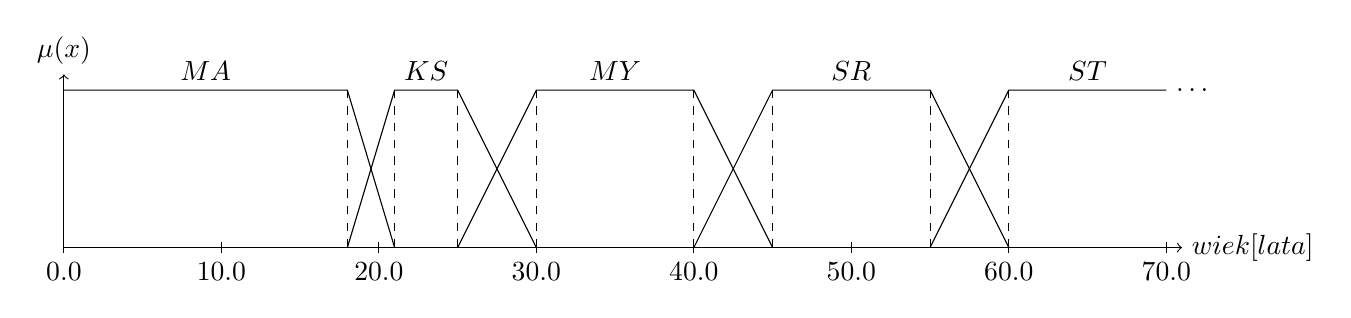
\begin{tikzpicture}[scale=2]
	\draw
		[->] (0,0) -- (0,1.1) node [anchor=south] {$\mu(x)$};

	\draw
		[->] (0,0) -- (7.1,0) node [anchor=west] {$wiek [lata]$};

	\foreach \x in {0,...,7}
		\pgfmathparse{\x*10}
		\pgfmathsetmacro{\age}{\pgfmathresult}
		\draw 
			(\x, 1pt) -- (\x, -1pt)
			node [anchor=north] {$\age$};

	\draw
		(0, 1) -- node [anchor=south] {$MA$} (1.8, 1) -- (2.1, 0);

	\draw [dashed]
		(1.8, 0) -- (1.8, 1);

	\draw
		(1.8, 0) -- (2.1, 1) -- node [anchor=south] {$KS$} (2.5, 1) -- (3.0, 0);

	\draw [dashed]
		(2.1, 0) -- (2.1, 1);

	\draw [dashed]
		(2.5, 0) -- (2.5, 1);

	\draw
		(2.5, 0) -- (3.0, 1) -- node [anchor=south] {$MY$} (4.0, 1) -- (4.5, 0);

	\draw [dashed]
		(3.0, 0) -- (3.0, 1);

	\draw [dashed]
		(2.5, 0) -- (2.5, 1);

	\draw [dashed]
		(4.0, 0) -- (4.0, 1);

	\draw
		(4.0, 0) -- (4.5, 1) -- node [anchor=south] {$SR$} (5.5, 1) -- (6.0, 0);

	\draw [dashed]
		(4.5, 0) -- (4.5, 1);

	\draw [dashed]
		(5.5, 0) -- (5.5, 1);

	\draw
		(5.5, 0) -- (6.0, 1) -- node [anchor=south] {$ST$} (7.0, 1) node [anchor=west] {$\ldots$};

	\draw [dashed]
		(6.0, 0) -- (6.0, 1);
\end{tikzpicture}

\caption{\label{fig:funkcja_we}Funkcja przynależności wieku (wejścia)}
\end{figure}

\begin{figure}[!h]
\centering
\begin{tikzpicture}[scale=1.5]
	\draw
		[->] (0,0) -- node [anchor=east] {$\mu(y)$} (0,1.6);

	\draw
		[->] (0,0) -- (10.1,0);

	\node at (5, -0.3) [anchor=north] {$wiarygodność [\%]$};

	\foreach \x in {0,...,10}
		\pgfmathparse{\x*10}
		\pgfmathsetmacro{\percent}{\pgfmathresult}
		\draw 
			(\x, 1pt) -- (\x, -1pt)
			node [anchor=north] {$\percent$};

	\draw
		(0.5, 0) -- (0.5, 1.5) node [anchor=south] {$OZ$} -- (1.5, 0);

	\draw
		(0.5, 0) -- (1.5, 1.5) node [anchor=south] {$M$} -- (6.6, 0);

	\draw [dashed]
		(1.5, 0) -- (1.5, 1.5);

	\draw
		(1.5, 0) -- (6.6, 1.5) node [anchor=south] {$S$} -- (10, 0);

	\draw [dashed]
		(6.6, 0) -- (6.6, 1.5);

	\draw
		(6.6, 0) -- (10, 1.5) node [anchor=south] {$D$} -- (10, 0);

	\draw [dashed]
		(6.6, 0) -- (6.6, 1.5);
\end{tikzpicture}

\caption{\label{fig:funkcja_wy}Funkcja przynależności wiarygodności (wyjścia)}
\end{figure}

\begin{figure}[!h]
\centering
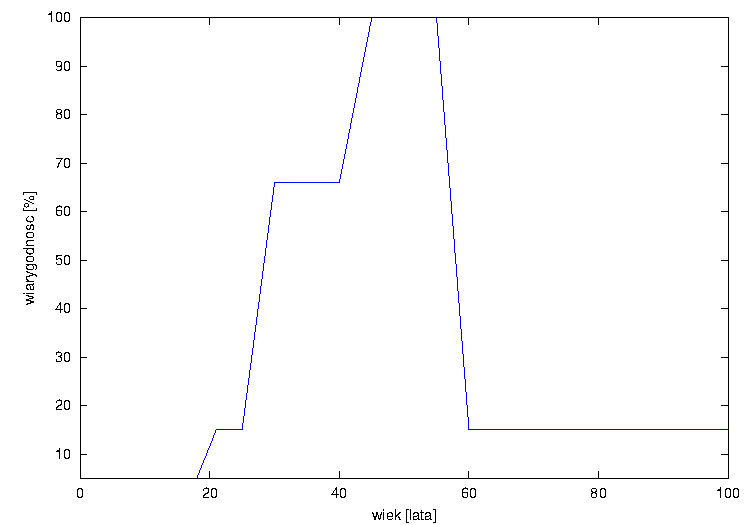
\includegraphics[scale=1.0]{src/char_wiarygodnosc.pdf}\caption{\label{fig:dane1}Charakterystyka systemu}
\end{figure}

\clearpage
\section{Nowoczesne sterowanie świateł pomocniczych}
W następującym przykładzie został zaprojektowany system z jednym wyjściem i dwoma wyjściami. W nowoczesnych samochodach można zauważyć "inteligentne światła pomocnicze". Te światła są montowane poniżej regularnymi światłami przednimi samochodu spełniające jednocześnie funkcje świateł przeciwmgielnych jak i świateł pomocniczych.

Światła pomocnicze włączają się automatycznie kiedy kierowca skręca kierownicą w lewo lub w prawo. Dzieje się tak kiedy kierowca chce skręcić w danym kierunku a światła pomocnicze mają wspomagać widoczność na lewej lub prawej stronie.

Wychylenie kierownicy jest mierzone w stopniach od pozycji jazdy prosto (0°). Wychylenie w lewo jest mierzone ujemnym kątem a wychylenie w prawo odpowiednio pozytywnym kątem. Światła pomocnicze są sterowane silnikiem elektrycznym i są w stanie wychylić się o maks. 30° w lewo lub prawo.

Aby nie oślepić kierowców z drugiego kierunku wychylenie w lewo świateł pomocniczych nie może wynosić więcej niż 10°. Kiedy kierowca chcę skręcić w prawo maksymalne wychylenie może wynosić 30°.

Kiedy kierowca jeździ prosto lub tylko lekko w lewo lub prawo, światła pomocnicze mają być wyłączone. Kiedy kierownica jest wychylona więcej niż 45° w prawo lub lewo światła mają się automatycznie włączyć.

Według powyżej podanych wymagań można zaprojektować system według następujących danych.

\begin{equation}
\begin{array}{ll}
x \in [-360, 360] & \textrm{We.: Wychylenie kierownicy w stopniach [°]} \\
y1 \in [-10,30] & \textrm{Wy.1: Wychylenie świateł pomocniczych w stopniach [°]} \\
y2 \in [0,100] & \textrm{Wy.2: Jasność świateł pomocniczych w procentach [\%]} \\
\end{array}
\end{equation}
\begin{center}Obszary rozwiązań na wejściu i wyjściu\end{center}

\begin{table}[h]
\centering
\begin{tabular}[t]{c|c}
Klucz & Pojęcie \\
\hline
LD & Lewo dużo \\
LSR & Lewo średnio \\
LM & Lewo mało \\
OZ & Około zera \\
PM & Prawo mało \\
PSR & Prawo średnio \\
PD & Prawo dużo \\
\end{tabular}
\caption{Słownik Wychylenia kierownicy (wejście)}
\end{table}

\begin{table}[h]
\centering
\begin{tabular}[t]{c|c}
Klucz & Pojęcie \\
\hline
LM & Lewo mało \\
OZ & Około zera \\
PM & Prawo mało \\
PS & Prawo średnio \\
PD & Prawo dużo \\
\end{tabular}
\caption{Słownik świateł pomocniczych (wyjście 1)}
\end{table}

\begin{table}[h]
\centering
\begin{tabular}[t]{c|c}
Klucz & Pojęcie \\
\hline
WY & Wyłączone \\
WL & Włączone \\
\end{tabular}
\caption{Jasność świateł pomocniczych (wyjście 2)}
\end{table}

\begin{table}[h]
\centering
\begin{tabular}[t]{c|c|c}
Wychylenie kierownicy & Wychylenie świateł & Jasność swiateł \\
\hline
LD & LM & WL \\
LSR & LM & WL \\
LM & LM & WL \\
OZ & OZ & WY \\
PM & PM & WL \\
PSR & PS & WL \\
PD & PD & WL \\
\end{tabular}
\caption{\label{tab:xor}Tabela reguł}
\end{table}

\begin{figure}[!h]
\centering
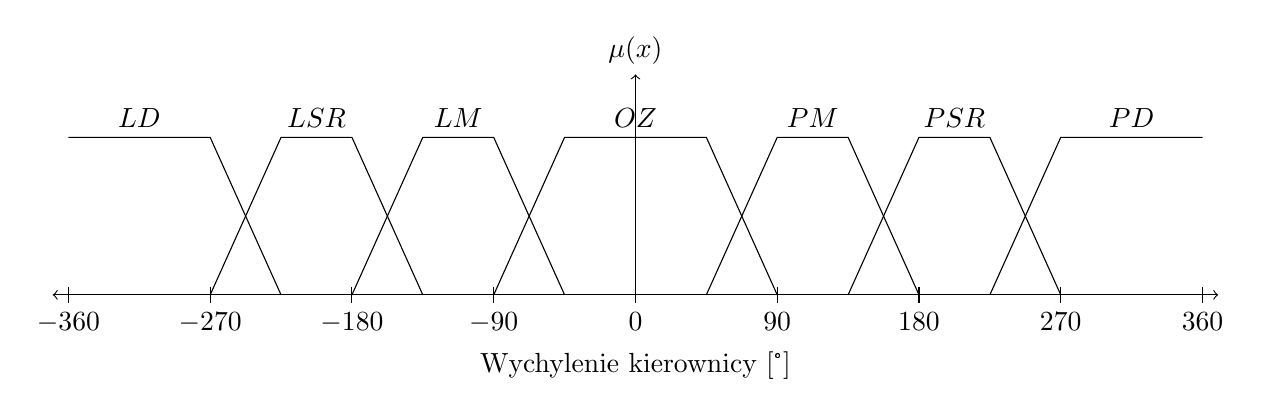
\begin{tikzpicture}[scale=0.02]
	\draw
		[->] (0,0) -- (0,140) node [anchor=south] {$\mu(x)$};

	\draw
		[<->] (-370,0) -- (370,0);

	\node at (0, -30) [anchor=north] {$\textrm{Wychylenie kierownicy [°]}$};

	\foreach \x in {-360,-270,-180,-90,0,90,180,270,360}
		\draw 
			(\x, 5) -- (\x, -5)
			node [anchor=north] {$\x$};

	\draw
		(-360, 100) -- node [anchor=south] {$LD$} (-270, 100) -- (-225, 0);

	\draw
		(-270, 0) -- (-225, 100) -- node [anchor=south] {$LSR$} (-180, 100) -- (-135, 0);

	\draw
		(-180, 0) -- (-135, 100) -- node [anchor=south] {$LM$} (-90, 100) -- (-45, 0);

	\draw
		(-90, 0) -- (-45, 100) -- node [anchor=south] {$OZ$} (45, 100) -- (90, 0);

	\draw
		(45, 0) -- (90, 100) -- node [anchor=south] {$PM$} (135, 100) -- (180, 0);

	\draw
		(135, 0) -- (180, 100) -- node [anchor=south] {$PSR$} (225, 100) -- (270, 0);

	\draw
		(225, 0) -- (270, 100) -- node [anchor=south] {$PD$} (360, 100);

\end{tikzpicture}

\caption{\label{fig:funkcja_we}Funkcja przynależności wieku (wejścia)}
\end{figure}

\begin{figure}[!h]
\centering
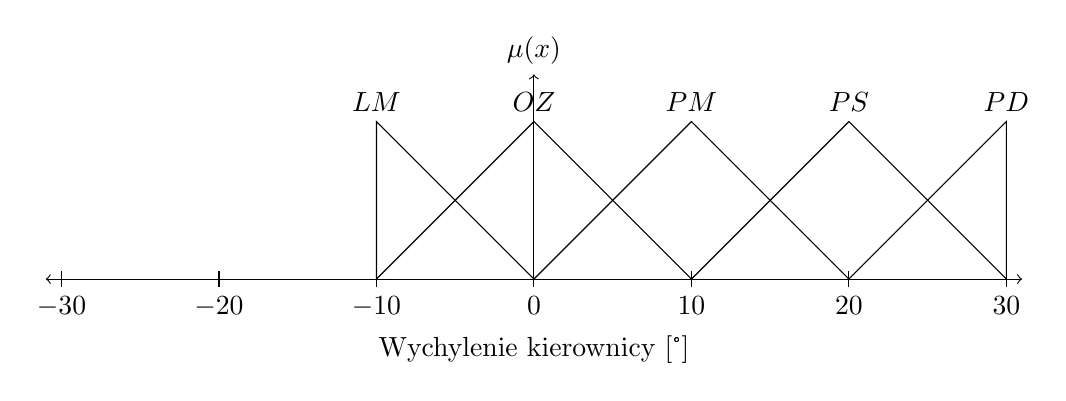
\begin{tikzpicture}[scale=0.2]
	\draw
		[->] (0,0) -- (0,13) node [anchor=south] {$\mu(x)$};

	\draw
		[<->] (-31,0) -- (31,0);

	\node at (0, -3) [anchor=north] {$\textrm{Wychylenie kierownicy [°]}$};

	\foreach \x in {-30,-20,-10,0,10,20,30}
		\draw 
			(\x, 0.5) -- (\x, -0.5)
			node [anchor=north] {$\x$};

	\draw
		(-10, 0) -- (-10, 10) node [anchor=south] {$LM$} -- (0, 0);

	\draw
		(-10, 0) -- (0, 10) node [anchor=south] {$OZ$} -- (10, 0);

	\draw
		(0, 0) -- (10, 10) node [anchor=south] {$PM$} -- (20, 0);

	\draw
		(10, 0) -- (20, 10) node [anchor=south] {$PS$} -- (30, 0);

	\draw
		(20, 0) -- (30, 10) node [anchor=south] {$PD$} -- (30, 0);
\end{tikzpicture}

\caption{Funkcja przynależności wieku (wejścia)}
\end{figure}

\begin{figure}[!h]
\centering
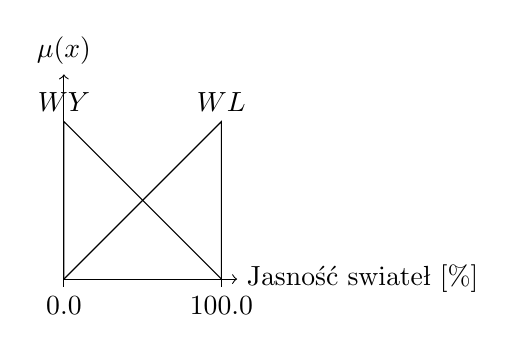
\begin{tikzpicture}[scale=0.2]
	\draw
		[->] (0,0) -- (0,13) node [anchor=south] {$\mu(x)$};

	\draw
		[->] (0,0) -- (11,0) node [anchor=west] {$\textrm{Jasność swiateł [\%]}$};

	\foreach \x in {0,10}
		\pgfmathparse{\x*10}
		\pgfmathsetmacro{\percent}{\pgfmathresult}
		\draw 
			(\x, 0.5) -- (\x, -0.5)
			node [anchor=north] {$\percent$};

	\draw
		(0, 0) -- (0, 10) node [anchor=south] {$WY$} -- (10, 0);

	\draw
		(0, 0) -- (10, 10) node [anchor=south] {$WL$} -- (10, 0);
\end{tikzpicture}

\caption{Funkcja przynależności wieku (wejścia)}
\end{figure}

\begin{figure}[!h]
\centering
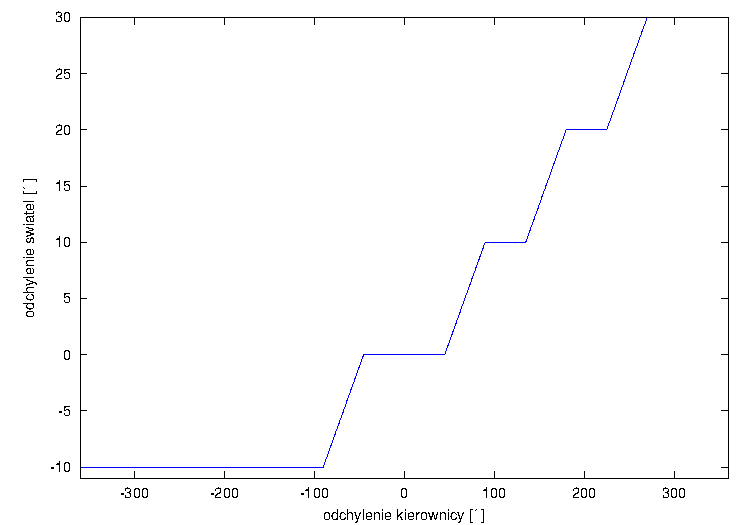
\includegraphics[scale=1.0]{src/char_swiatla.pdf}\caption{\label{fig:dane1}Charakterystyka systemu}
\end{figure}

\begin{figure}[!h]
\centering
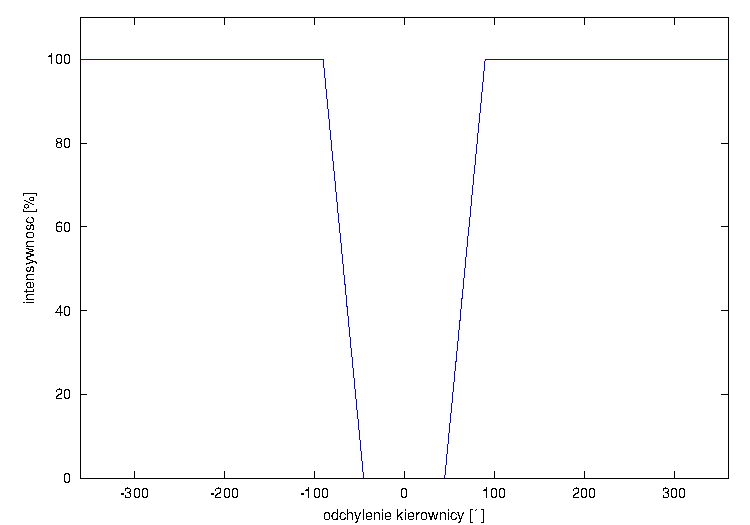
\includegraphics[scale=1.0]{src/char_swiatla_intensywnosc.pdf}\caption{\label{fig:dane1}Charakterystyka systemu}
\end{figure}

